\documentclass[12pt,a4paper]{article}
\usepackage{mystyle}
%\usepackage{schueler}
%\usepackage{lehrer}

\usepackage{circuitikz}


\author{}
\date{}
\title{Abbildungen mit Linsen}

\begin{document}
\maketitle
%\thispagestyle{empty}

\section*{Material}
Für diesen Praktikumstag werden folgende Materialien benötigt:
\begin{itemize}
	\item Optische Bank mit Lampe und Linsen 
	\item Experimentiertischchen
	\item Transformator
\end{itemize}

\section*{Vorbereitung und Versuchsaufbau}

\begin{itemize}
	\item Entfernen Sie alle Komponenten ausser der Lampe von der optischen Bank.
	\item Verbinden Sie Lampe und Transformator und schalte Sie damit die Lampe ein.
	\item Montiere Sie ein Linse (mit positiver Brennweite) vor der Lampe.
	\item Stellen Sie das Experimentiertischchen als Schirm vor die Linse.
\end{itemize}


\begin{figure}[t]
	\begin{center}
	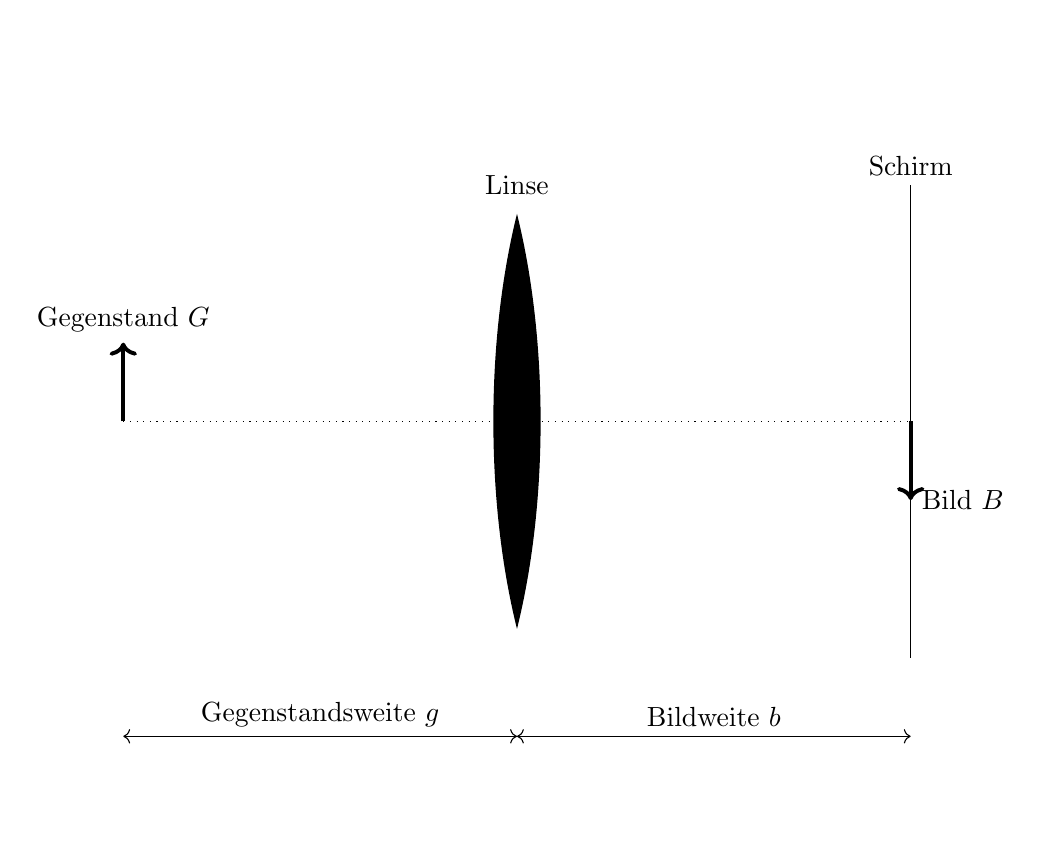
\begin{tikzpicture}

%Mittellinie
\draw [dotted] (-5,0)--(5,0);

%Gegenstand
\draw [->=latex, line width=0.05cm] (-5,0)--(-5,1) node [above] {Gegenstand $G$};
%Bild
\draw [->=latex, line width=0.05cm] (5,0)--(5,-1) node [right] {Bild $B$};

\begin{scope}[xscale=2, yscale=5]
\clip (-0.85,0) circle (1cm);
\clip (0.85,0) circle (1cm);
\fill(-2,-2) rectangle (2,2);
\end{scope}

\draw (0,3) node {Linse};

%Schirm
\draw (5,-3)--(5,3) node [above] {Schirm};


\draw [<->=latex] (-5,-4)--(0,-4) node [midway, above] {Gegenstandsweite $g$};
\draw [<->=latex] (0,-4)--(5,-4) node [midway, above] {Bildweite $b$};
\end{tikzpicture}
	\caption{\label{fig1} Skizze des Versuchsaufbaus.} 
	\end{center}
\end{figure}



\section*{Versuch}
\begin{itemize}
	\item Der Glühdraht der Lampe ist der Gegenstand $G$.
	\item Suchen Sie das Bild des Gegenstandes, verändern Sie dazu Gegenstandsweite $g$ und Bildweite $b$.
	\item Wie ist die Vergrösserung?
	\item Versuchen Sie systematisch Zusammenhänge zwischen $B/G$ und $b/g$ zu finden (Tabelle).
	\item Tragen Sie die reziproke Bildweite $1/b$ über der reziproken Gegenstandsweite $1/g$ auf (Graph).
	\item Wiederholen Sie den Versuch mit einer Linse mit anderer positiver Brennweite.
\end{itemize}

\section*{Zusammenfassung}
\begin{itemize}
	\item Was haben Si im Praktikum gemacht?
	\item Welcher Zusammenhang besteht zwischen $B/G$ und $b/g$ bei Linsen?
	\item Konnten Sie die Linsenformel
		\begin{eqnarray*}
			\frac{1}{f} = \frac{1}{b} + \frac{1}{g}
		\end{eqnarray*}
bestätigen?
\end{itemize}

\end{document}
